\chapter{Szervezeti alapvetések}
\section{Szervezet architektúrája}

% forras: https://mindsetpszichologia.hu/2017/11/29/fonok-nelkul-szabadon-a-holacracy-nyomaban/

Az iskolák hagyományosan hierarchikus vezetési és munkaszervezési elveket követnek. Főnök-beosztott viszonyok, felülről jövő döntések és autoritás határozza meg a mindennapi folyamatokat. Az állandóság és a biztos siker érdekében ezek az iskolák a centralizált hatalmat alkalmazzák: a főnök dönt, a beosztottak végrehajtanak. A Budapest Schoola a mai világra reflektálva egy dinamikusabb, gyors változásokat támogató modellt dolgozott ki az egyes mikroiskolák hatékony és mégis decentralizált működtetésére.

Olyan kihívásokra reflektál ez a működési mód amelyek nagyobb komplexitást, transzparenciát és szélesebb körű kommunikációs lehetőségeket kívánnak meg. Így rövidülhet a döntéshozatal, a gazdasági, a környezetet és a tanulás körülményeit érintő kérdésekben pedig növekszik az érintettek felhatalmazása és bevonódása. A Budapest School egy olyan mikroiskolai modell működtetését határozza meg, amely önfenntartó, környezettudatos és etikus. Támogatja a munkavállalók kreativitását és lelkesedését és egy agilis, gyorsan változó és fejlődő szervezet épülését segíti.


\section{A Budapest School szervezeti modellje, szociokrácia}

A szociokrácia egy olyan új „szociális technológiát” biztosít a szervezetek irányítására és működtetésére, amelyet a hagyományos, hierarchikus szervezetektől eltérő alapvető szabályok határoznak meg.

Egy öngazdálkodó gyakorlat a célirányos és változásra fogékony szervezeteknek.

A megközelítés – az agilis és lean megoldásokhoz hasonlóan – „just in time”, vagyis épp a kellő pillanatban reagál a felmerülő változásokra és lehetőségekre. Mindezt pedig a vállalat minden szintjén önállóan teszi.

Az iskolai szervezet alapelemei a következők:
\begin{itemize}
    \item egy keretrendszer, ami lefekteti a „játékszabályokat” és újraosztja a hatalmat,
    \item egy módszer a szervezet újrastrukturálásához és az emberek szerepeinek és önállóságának meghatározásához,
    \item egy egyedülálló döntéshozatali folyamat a hagyományos döntési folyamatok felfrissítéséhez,
\end{itemize}

\section{Dinamikusan változó szerepek}

A klasszikus iskolában minden alkalmazott rendelkezik egy munkaköri leírással, mely felsorolja feladatait és hatáskörét. Ez általában a legkevésbé sincs összhangban a nap mint nap végzett feladatokkal. A Budapest School iskálban a dolgozók gyakran számos szereppel rendelkeznek, ezek pedig lehetnek akár teljesen különböző munkacsapatokon belül is. A szerepek folyamatos alakuláson mennek keresztül és frissülnek a csapat résztvevői által. Egy szerepkör tehát nem lesz szorosan egy emberhez kapcsolva: mindig az látja majd el, aki ért hozzá, van szabad kapacitása és elvállalja. Ezzel pedig sok személyes konfliktus kerülhető el. Ahogy például
\emph{a fociban is pontosan tudod, hogy a labdát a csatárnak kell passzolnod}.

Nem azért, mert jóban vagytok, hanem mert ő van a legjobb helyzetben, hogy gólt lőjön a csapatnak. Még ha nem is vagy vele jóban, nem kedveled vagy ki nem állhatod, akkor is neki fogsz passzolni, mert a játék stratégiája szerint így kell tenned. Ugyanígy az iskolánkban az egyes szerepek rendelkeznek hatalommal, nem pedig a személyek. Ez azt is jelenti, hogy a szerepek és a hatalom állandóan változhatnak anélkül, hogy a játékszabályokat megsértenénk. Nincs állandó főnök-beosztott viszony.

\section{Szétosztott hatalom}

A hagyományos iskolai struktúrában az igazgató és a vezetőség tagjai nem delegálnak hatalmat. Minden döntés az ő kezeik között folyik át. A Budapest School iskolában a hatalom ténylegesen elosztásra kerül, így a hierarchia helyett egymással kapcsolatban lévő és kommunikáló, de önállóan döntő csapatok (úgynevezett körök) a döntéshozók. A körök közötti kapcsolat jelentősen meg tudja növelni az iskolai kapacitást az alkalmazkodáshoz.

\section{Állandó tyúklépések}

Budapest School iskolában a szervezeti struktúra minden hónapban felülvizsgálásra kerülhet: megvizsgálják, hogy az adott szerepek milyen feladatokkal és döntésekkel járnak. A változások tömérdek apró lépésben történnek, szünet nélkül, folyamatosan. Így a csapat kihasználhatja a lehetőségeket, hogy tanuljon az esetleges hibákból, fejlessze önmagát és tökéletesítse a folyamatokat. Ahogy Alexis Gonzales-Black, a Zappos munkatársa mondja (akik talán a legelsők között csatlakoztak a holacracy átültetéséhez), „a holacracy nem fogja megoldani helyetted a problémáidat; viszont egy jó eszköz arra, hogy te megoldhasd őket saját magadnak.”

\section{Mindenki számára átlátható szerepek}

„Mi mindig így csináljuk” – hangzik el számos iskolánál a válasz, hogy ez vagy az miért éppen így történik. Gyakran senki sem tudja, hogy az adott szabály miért létezik, mi célt szolgál, ki döntött róla vagy ki tudná megváltoztatni. Ez pedig a hatalom szétosztását lehetetlenné teszi. A Budapest School iskolában

\emph{a hatalom nem a csoport élén álló vezetők kezében van,}

hanem az expliciten definiált folyamatokhoz kötődik. Ezek a „játékszabályok” mindenki számára elérhetőek és ismertek, legyen szó akár régi motorosokról, akár az újoncakról.

A Budapest School modellel tehát nem káoszt és hatalmi játszmákat generálunk, hanem

\emph{eltöröljük a hagyományos hierarchiából fakadó lassú folyamatokat,}

az átláthatatlan felelősségi köröket és szabad utat engedünk a kreativitásnak, az önállóságnak. Azáltal, hogy felhatalmazza az embereket arra, hogy értelmes döntéseket hozhassanak és részt vehessenek a változásban, a holakrácia felszabadítja a szervezet kihasználatlan erőforrásait.



\section{Az iskola kormányzása}
\label{sec:az_iskola_kormanyzasa}
Az iskola szervezetét a tagjai együtt alakítják. A szervezet élő, folyamatosan változik, a következő alapelvek mentén:

\begin{itemize}

  \item
        Gyorsan és folyamatosan tanuló, agilis szervezetként az iskola min\-den\-nap jobban támogatja a gyerekek tanulását, mint tegnap.
  \item
        Minden résztvevő stabilitás, biztonság, kiszámíthatóság iránti igénye pont annyira fontos, mint a változás, a javulás, a fejlődés igénye.
  \item
        A gyerekeket leginkább ismerő, hozzájuk legközelebb álló tanárok (gyerekekkel és szülőkkel erős kapcsolatban) minél több helyzetben hoznak döntéseket.
  \item
        Az együttműködés, a partneri kapcsolat, a kölcsönös felhatalmazás a tanárok, adminisztrátorok között is folytonos, nem csak a tanár-gyerek kapcsolatban.
\end{itemize}

Azt szeretnénk, hogy gyerekeink kreatív, környezetüket aktívan alakító, mély partneri kapcsolatokban élő, problémamegoldó, csapatjátékos, folyamatosan tanuló, a világot változtatni tudó felnőttekké váljanak. Ehhez olyan iskolát építünk, ahol a tanárok kreatívak, környezetüket aktívan alakítják, mély partneri kapcsolatban élnek, problémákat oldanak meg, csapatban dolgoznak és folyamatosan tanulnak.

Az iskolát mint szervezetet a \emph{szociokrácia} (sociocracy) szervezeti modell alapján működtetjük, mert így tudjuk leginkább elérni, hogy egyszerre legyen örömteli és hatékony az együttműködésünk. Ez egy olyan, az üzleti világban is kipróbált dinamikus döntéshozatali rendszer, amely egyszerre segíti a harmonikus és örömteli közösségi együttműködést, és jelent garanciát arra, hogy az együttműködés hatékony lesz az egyes csapatokon belül.

\subsection{Döntéshozás}
\label{sec:consent_based}

Az iskola minden csapata (egy mikroiskolát működtető tanulásszervezők, gyerekek egy csapata stb.) a \emph{hozzájáruláson alapuló döntési mechanizmust} (consent based decision making) használja ahhoz, hogy a szervezet gyorsan tudjon döntést hozni, \emph{és} minden tagja hallathassa a hangját.

A csapat valamennyi tagja hozhat javaslatokat, ha működési
hatékonytalanságot, feszültséget, problémát talál, és van rá
megoldása. A javaslat értelmezése után az érintettek mindegyikét meg
kell hallgatni, hogy \emph{elfogadhatónak} tartja-e a javaslatot, azaz
hozzájárul-e a változáshoz, mert \emph{,,elég jónak és biztonságosnak
  találja, hogy kipróbáljuk az új működést''} (\emph{``is this
  good enough for now and safe enough to try?''}). Fontos, hogy
mindenki egyenként hallassa hangját. A javaslat elfogadásra kerül, ha
és amikor minden érintett hozzájárult.

Mindenki kifejezheti a \emph{fenntartásait} (concern), és a csapat feladata ezeket meghallani, és reagálni rájuk. A fenntartás azonban még nem jelenti a javaslat elutasítását, csak fontos információt ad a döntés végrehajtásához.

A javaslatot a csapat nem fogadja el, ha valamelyik csapattag \emph{ellenzi} (objection) azt. Az ellenzés egy én-üzenet, valami olyasmi: ,,ha a csapat ezt a döntést meghozná, akkor mélyen sérülne a csapathoz való elköteleződésem, mert az én igényemet, ami \ldots{}, nem elégíti ki a javaslat. Nekem szükségem van \ldots{}, ezért inkább javaslom, hogy \ldots{}''. Fontos, hogy az ellenvetést megfogalmazó mondja el a saját igényeit, szükségleteit és tegyen új javaslatot, vagy kérjen segítséget, hogy milyen új javaslatot tehetne. Ellenvetés esetén a csapat együtt dolgozik azon, hogy új javaslatot találjon, ami az ellenvetést feloldja, és az eredeti javaslat célja felé viszi a szervezetet.

\paragraph{A hozzájárulás nem konszenzus}

A konszenzus alapú döntések esetén mindenkinek egyet kell értenie abban, hogy a döntés a legjobb, leghelyesebb, leghelyénvalóbb. A Budapest School iskolában azt a kérdést tesszük fel inkább, hogy van-e valakinek ellenvetése és a javaslat kellően biz\-ton\-sá\-gos-e ahhoz, hogy kipróbáljuk. Nem azt a kérdést tesszük fel, hogy mindenki ezt a döntést hozta volna-e és mindenki egyetért-e a döntéssel hanem azt, hogy mindenki tudja-e támogatni a csapat egy másik tagját, és nincs-e olyan ismert kockázat, ami az egyén vagy a szervezet szempontjából nem vállalható fel.

\paragraph{A hozzájárulás nem szavazás}

A Budapest School iskolában nem a többség dönt, és nem az számít, hogy hányan akarnak egy döntés mellé állni. Mindenki hozhat döntést, amit elfogad a csapat minden tagja, azaz egyetlenegy ellenvetés sincs.

\paragraph{Az ellenvetés nem vétó}

A vetójog gyakorlatban a döntés megakadályozását jelenti. Amikor valaki megvétóz egy döntést, akkor azzal a folyamat általában megakad. Az iskola működésében használt ellenvetés egy beszélgetés megindítását jelenti: ,,ezt én így nem tudom támogatni, helyette ezt javaslom inkább''.

\paragraph{A ,,van egy jobb ötletem'', nem ellenvetés}

A szervezetnek nem az a feladata, hogy a legjobb döntéseket hozza, hanem hogy amikor szükséges, akkor javítson a működésén. Ezért minden döntéskor mindenkinek azt kell mérlegelnie először, hogy elfogadható-e neki, hogy azt a bizonyos javaslatot kipróbálja a csapat. Attól, hogy valaki jobb, más javaslatot is tud, attól még először az eredeti javaslatot érdemes kipróbálni és tesztelni.

\paragraph{Minden javaslat csak egy hipotézis}

Amikor valamit változtatunk a szervezet működésén, akkor egy kísérletbe vágunk bele: kipróbáljuk, hogy az új működés tényleg jobb-e, megoldja-e a problémát, feszültséget, kielégí\-ti-e az igényeket. A döntés támogatásakor ezt a próbálkozást támogatjuk.

\paragraph{Nem döntünk mindenről együtt}

A Budapest School iskolá\-ban csak az iskola és a mikroiskola működését megváltoztató kormányzási kérdésekről döntünk együtt.~A Budapest School minden tagja szerepeiből kifolyólag fel van hatalmazva arra, hogy a mindennapi döntéseit maga meghozhassa, ezért nem kell mindent megbeszélnünk. A cél, hogy olyan szerepeket és rendszereket alakítsunk ki, hogy a mindennapi döntéseket mindenki maga meg tudja hozni.

\subsection{Csapatok -- az iskola szervezeti egységei}

A Budapest School csapatai (a szociokrácia terminológiájában a \emph{körök}) önálló csoportok egy jól meghatározott céllal, felruházott felelősséggel, döntési körrel. A csapatok maguk határozzák meg a saját működésüket (policy making), és végzik el a saját feladatukat. Az iskolában azok döntenek együtt, akik együtt dolgoznak, egy csapatban (``those who associate together govern together''). És fontos, hogy akik együtt dolgoznak, jól legyenek egy\-mással.

Azt is tudjuk, hogy akik egy munkát elvégeznek, azok a munka szak\-ér\-tői, ezért ők tudnak arról a legjobban dönteni, hogy hogyan érdemes a munká\-ju\-kat szervezni, alakítani. Nincs főnök, külső szakértő, aki megmondja egy csapatnak, mit és hogyan csináljanak addig, amíg a rájuk felhatalmazott kereteken belül maradnak. Az természetes, hogy minden segítséget, támogatást, információt megkapnak, amire szükségük van. De a kormányzás az ő kezükben van.

\paragraph{Mikroiskola tanulásszervező csapata.}

A Budapest School szervezet állandó csapatai az egy-egy mikroiskolát vezető tanulásszervezők csapata, ami egy \emph{szociokratikus kör}. A mikroiskola gyerekeinek (családjainak) és tanárainak életét meghatározó döntéseket maguk hozzák meg. Így például a napirend, a csoportbontások, a szülői értekezletek tematikája a saját döntéseik alapján alakul ki. Fontos, hogy a csapattagok maguk tudják meghatározni, kivel tudnak és akarnak együtt dolgozni, mikor és mit akarnak csinálni.

\paragraph{Csapatok kapcsolódása}

Egy-egy ember több csapatnak is tagja lehet. Egyrészt munkacsoportok alakulhatnak egy-egy feladat elvégzésére, és a Budapest Schoolban egy ember több részfeladatot is ellát. Másrészt a csapatokat kifejezetten úgy alakítja a közösség, hogy legyenek köztük kapcsolódások, olyan tagok, akik összekötik a csapatokat.

Vannak olyan csapatok, melyek elsődleges célja összekötni a kisebb csapatokat. Például minden mikroiskolai csapat delegál egy képviselőt az iskola közös naptárát létrehozó munka\-csoportba.

\paragraph{Csapatok vezetői}

Minden csapatnak van egy \emph{vezetője} (szociokrácia terminológiában a
\emph{circle leader}). A vezető feladata, hogy mindenki ismerje a csapat célját, a \emph{,,miért létezünk?''} kérdésre a választ, és hogy a csapat működjön: tiszták legyenek a szerepek és megtörténjen az, amiben megállapodott a csapat, és működjenek és fejlődjenek a folyamatok.

A csapatvezető a Budapest School rendszerében nem az, aki
meg-\linebreak
mondja, ki mit csináljon, nem osztja, ellenőrzi vagy felügyeli a feladatokat, nem rúg ki, és nem vesz fel embereket, hanem szolgálja a csapatot (servant leadership) azzal, hogy segíti a megállapodásokat betartani: facilitál, moderál, szintetizál, kísér, kérdez. A csapatvezető megválasztásához, mint minden szerep megválasztásához, a csapat minden tagjának hozzájárulása szükséges.

% Strukturál, összeszervez, koordinál, levezet, emlékeztet.

%Learning architect
%ne legyen bystander
%Ő sem autoritas,  hanem javasol, tematizál, szempontot hoz.

%az, aki arról beszél, hogy a gyerekek igyényeinek milyen struktúrák, keretek, %csoportbontások, modulok, tevékenyslg felelnek meg leginkább 

\subsection{Mi van, amikor egy csapat nem tud döntést hozni,\\ együttműködni?}

Amikor a csapattagok úgy érzik, hogy nem tudnak mindenki számára elfogadható döntéseket hozni, nem haladnak, vagy megjelentek a játszmák, és ezért már nem tudják a csapat célját szolgálni, akkor konfliktus, feszültség alakul ki, aminek feloldásához segítséget hívhatnak be a szervezet töb\-bi részétől. %(lásd .~fejezet).

A csapat folyamatos harmóniájáért folyamatosan dolgozni kell, ahogy az egészségünk megőrzése és a problémák megelőzése is napi rutinná kell hogy váljon. Ezért a Budapest School csapatainak erősen ajánlott a rendszeres visszajelzés, visszatekintés (retrospektív) és a team coaching.

 
\begin{figure}[htb]
    \begin{center}
    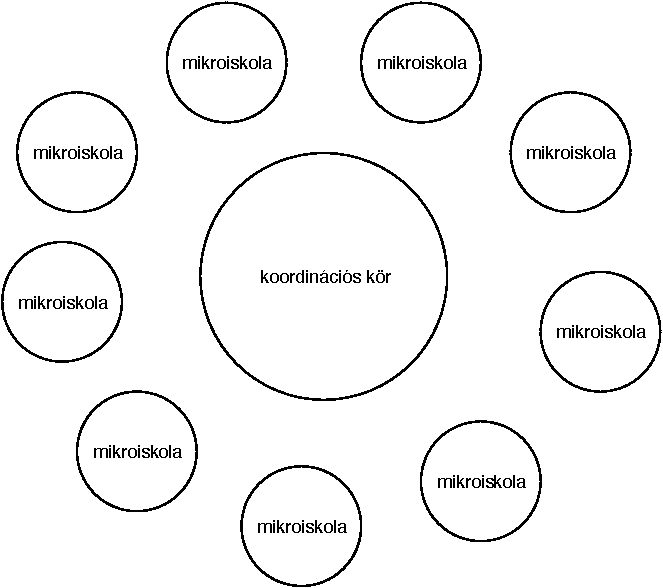
\includegraphics{chapters/szmsz/org_chart.pdf} 
    \end{center}
    \caption{A Budapest School szervezeti diagramja nem egy hagyományos hierarchikus szervezetet mutat, hanem önállóan működő köröket. A szervezetet a mikroiskolák koordinációs vezetői fogják össze. }
\end{figure}

\section{A közösségi lét szabályai}
\label{sec:kozossegi_elet}
A Budapest School egy közösségi iskola: a gyerekek együtt tanulnak és alkotnak, a tanárok csapatokban dolgoznak és a szülők is egy elfogadó közösség részének érezhetiek magukat. A tagok -- a tanárok, a gyerekek, a szülők, és az adminisztrátorok -- azért csatlakoznak a közösséghez, mert itt szeretnének lenni és itt érzik magukat boldognak, egészségesnek és hasznosnak. A közösség azért fogad be új tagokat, hogy nagyobb, erősebb közösség tudjunk lenni.

\paragraph{Alap csoportok} A Budapest School iskola kisebb mikroiskolák
hálózataként működik (lásd \aref{sec:mikroiskola} fejezetet). Ez a gyerekek és tanárok elsődleges közössége: gyerekként ez az a közösség, akikkel együtt járok iskolába, együtt alakítom az iskolámat, tanárként ez az a csapat, akikkel együtt dolgozom, hogy létrehozzuk, tarsuk és fejlesszük a mikroiskola gyerekeinek tanulási környezetét.

A tanulás egysége a modul, amiről \aref{sec:modulok} fejezet részletesen ír. Egy modul csoportjában a közös érdeklődésű és célú gyerekek tanulnak együtt, mert együtt boldogabban, hatékonyabban el tudják érni a céljukat.

\paragraph{Saját szabályok}
\label{sec:sajat_szabalyok}
A mikroiskola és akár egy-egy modul kereteit, szabályait a résztvevők alakítják ki. Pontosabban a tanárok \footnote{Mikroiskola esetén a tanulásszervező tanárok, modulok esetén a modulvezető tanárok és a tanulásszervező tanárok közösen.} felelőssége és feladata, hogy mindenk tanár és gyerek számára elofgadható, betartható, releváns és értelmes szabályok legyenek. Mind a gyerekek, mind a tanárok javasolhatnak új szabályokat, vagy szabályváltoztatást. Minden egyes gyereknek és tanárnak hozzájárulását kell adnia minden javaslathoz, mondván: ,,it's good enough for now and safe enough to try", azaz, ,,elég jónak és biztonságosnak tartom, hogy kiprobáljuk'' a szabályokat.

Ebből következik, hogy minden mikroiskolának saját házirendje, szabályai lehetnek, és modulonként alakulhat, hogy mit, mikor, hogyan és kivel csinálnak a résztvevők.

Szabályok alakításának elsődleges szándéka mindig az legyen, hogy hogy a gyerekek fejlődése, tanulása, alkotása és a közösség működése egyre jobb legyen.

\subsection{Konfliktusok, feszültségek kezelése}
\label{sec:konfliktusok_kezelese}
Tudjuk, hogy a Budapest School szereplői, a gyerekek, a tanárok, a szülők, a pedagógia program, a kerettanterv, a fenntartó, a szomszédok, az állami hivatalok  között feszültségek és konfliktusok alakulhatnak ki, mert különbözőek vagyunk, különbözőek az igényeink. A feszültségekre és a konfliktusokra a Budapest School olyan lehetőségként tekint, amelyek együttműködésen alapuló megoldása építi a kapcsolatot, és segíti a fejlődést.

Minden vágy, ötlet, szándék, cél, viselkedés közötti különbség, ha az valamelyik félben negatív érzéseket kelt, feszültséget és konfliktus okozhat. Ebbe beletartozik az is, ha valaki nem azt és úgy csinálja, ahogy nekünk erre szükségünk van, vagy ha bármilyen okból nem érezzük magunkat biztonságban, vagy más univerzális emberei szükségletünk \citep{rosenberg2003nonviolent} nem elégül ki.

Konfliktus alakulhat ki a gyerekek, szülők és tanárok között bármilyen relációban és adódhatnak egyéb, belső konfliktusok, nehézségek is akár a család, akár a Budapest School életében, amelyek kihathatnak a közösségi kapcsolatainkra.

\subsubsection{A BPS konfliktusok feloldása}

Az iskola a partnerségen alapuló szervezetében nem autoritások, főnökök, hivatalok, bírók oldják meg a konfliktusokat, hanem egyenrangú társak. Az iskola feltételezi, hogy a felek tudnak gondolkodni, következtetni, felelősséget vállalni a döntéseikért és cselekedetikért.\footnote{Kisgyerekeket mentoraik és szüleik reprezentálnak.}

\paragraph{Alapértékek}
Ahhoz, hogy tényleg partneri kapcsolatban, egyenrangú felekként tudjunk konfliktusokat, problémákat megoldani, érdemes közös értékeket elfogadni.
\begin{itemize}
      \item Először a saját változásunkon dolgozunk, mert nem nagyon tudunk mást embert megváltoztatni, csak magunk változásáért lehetünk felelősek.
      \item Felelősséget vállalunk gondolatainkért, hiedelmeinkért, szavainkért és viselkedésünkért.
      \item Nem pletykálunk, szóbeszédet nem terjesztjük.
      \item Nem beszélünk ki embereket a hátuk mögött.
      \item Félreértéseket tisztázunk, konfliktusokat felszínre hozunk.
      \item Személyesen, 1-on-1 beszélünk meg problémákat, másokat nem húzunk be a problémába.
      \item Nem hibáztatunk másokat a problémákért. Amikor mégis, akkor az egy jó alkalom arról gondolkozni, hogy miként vagyunk mi is része a problémának, és kell a megoldás részévé vállnunk.
      \item Erősségekre több figyelmet fordítunk, mint a gyengeségekre, és a lehetőségekről, megoldásokról többet beszélünk, mint a problémákról.
\end{itemize}

\paragraph{Feszültségre felszínre hozása}
Olyan módszereket, folyamatokat, szabályokat, szokásokat kell kialakítani minden közösségben, hogy legyen tere és ideje a feszültségeket előhozni.
\begin{itemize}
      \item Iskolai csoportok rendszeresen kezdik a napjukat egy bejelentkező körrel, ahol van lehetőség a feszültségeket is felhozni.
      \item A csoportok rendszeresen tartanak retrospektív gyűlést, ahol értékelik, mi volt jó és nem annyira jó egy vizsgált időszakban.
      \item Évente legalább kétszer a tanárok egymásnak, a szülők a tanároknak, a gyerekek a tanároknak, a tanárok a gyerekeknek visszajelzést adnak szervezett formában.
      \item A gyerekek a mentorukkal rendszeresen találkoznak, ahol teret kapnak a felmerülő feszültségek.
\end{itemize}

\paragraph{Megbeszélés}

A Budapest School közösségének valamennyi tagja (a tanárok, gyerekek, szülők, adminisztrátorok, iskolát képviselő fenntartó) vállalja:

\begin{itemize}

      \item A közösség mindennapjaival kapcsolatos konfliktusok esetén elsőként az abban érintett személynek jelez közvetlenül.
      \item Személyes kritikát mindig privát csatornán fogalmazza meg először, ha kell, akkor segítő bevonásával.
      \item   Bármelyik fél jelzése esetén lehetőséget biztosít arra, hogy a vitás kérdést megbeszéljék közvetlenül, a folyamatban részt vesz.
      \item
            Szakítás, kilépés, lezárás előtt legalább három alkalommal megpróbál egyeztetni.
      \item
            Az egyeztetésre elegendő időt hagy, amely legalább 30 nap vagy -- amennyiben több időre van szükség -- a másik féllel megállapodott idő.
      \item
            Teljes figyelemmel, nyitottsággal, a probléma megoldására fókuszálva igyekszik feloldani a konfliktust, és közösen megoldást találni a problémára.
\end{itemize}

Összefoglalva: ha problémánk van egymással, akkor azt megbeszéljük. Nem okozunk egymásnak meglepetést, mert vállaljuk, hogy rögtön elmondjuk egymásnak konfliktusainkat.

\paragraph{Közvetítő bevonása}

Ha úgy érezzük, hogy a személyes egyeztetés nem vezetett megoldásra, a tárgyalást külső segítség bevonásával folytatjuk. Ez lehet egy másik csoporttag, egy tanár, vagy egy teljesen külsős meditátor.

Amikor bármely fél közvetítőt kér, akkor a másik ezt elfogadja. Nem mondhatjuk azt, hogy  \emph{,,de hát mi magunk is meg tudjuk oldani a konfliktust''}.

\paragraph{Eszkalálás}

Ha két fél nem tudja megoldani a konfliktust, akkor kérhetnek segítséget a \texttt{segitseg@budapestschool.org} címen, amire 48 órán belül kell válaszolnia. Az email kezeléséért az iskola igazgató felel.

\paragraph{Megállapodások}

Ha az egyeztetés, tárgyalás és közvetítő bevonása során sikerül valamilyen megoldást vagy a megoldáshoz vezető folyamatot egyeztetni, a felek \emph{megállapodnak} abban, hogy ki mit tesz, vagy milyen szabályokat alakítanak ki, illetve, hogy mennyi időt adnak egymásnak, hogy kipróbálják, sikerült-e feloldani a konfliktust. Segíteni szokott a kérdés, hogy \emph{most megállapodtunk vagy csak beszéltünk róla?}, hogy minden fél számára világos legyen a megállapodás.

Nagyobb konfliktusok esetén jó gyakorlat, és bármely fél kérheti, hogy írásban is rögzítsék a megállapodást. Ez lehet egy papirfecni is, vagy egy email. Lényege nem a formátum, hanem  hogy minden fél emlékezzen a megállapodásra.

\paragraph{Egyeztetés sikertelen}

Ha a felek között az egyeztetés sikertelen volt, vagy a megoldási javaslat nem működött, a felek ezt írásban meg kell, hogy állapítsák. Erre azért van szükség, hogy egyetértés legyen abban közöttük, hogy értik, a másik fél sikertelennek érzi az egyeztetést.

\paragraph{Lezárás}

Az egyeztetés sikertelensége esetén elengedjük egymást. De ez a végső megoldás.

\subsection{Kiemelt konfliktusok}

\subsubsection{Gyerek-gyerek konfliktus}

A mindennapokban a gyerekek akarva akaratlanul belecsöppennek olyan hely\-ze\-tek\-be, amikor a közösségben vagy interperszonális kapcsolataik során megborul a mindennapi egyensúly. Ezekben a konfliktushelyzetekben leginkább a felborult egyensúly helyreállítására törekszünk \emph{resztoratív konfliktusfeloldási technikával}.

A resztoratív konfliktusfeloldás alaptézise az, hogy minden ilyen megborult egyensúlyi állapot egy lehetőség valami megújítására, újragondolására. A résztvevők egy külső személy segítségével (általában a jelenlévő tanár) együtt alakítják a megoldást, egészen addig, amíg az eredmény mindenki számára a konfliktus feloldását jelenti, azaz a megborult egyensúly helyreállítását.

A folyamat során a konfliktusban résztvevő összes személy elmondja az érzéseit, meglátását a felmerülő helyzettel kapcsolatban, valamint az én-közléseken túl a szükségleteikről is beszélnek. Ezen szükségletek képezik a megoldás alapját, azaz ezeket egy tető alá hozva feloldhatjuk a fennálló konfliktust. Ilyenkor mindig először azokat a pontokat keressük meg, amelyekben egyetértenek a résztvevők, hiszen ez egy közös alapot szolgáltat arra, hogy a valódi feloldást megtalálhassuk.

Fontos, hogy a beszélgetésben az összes fél hallassa a hangját, és meg is legyen hallgatva. Az értő figyelem kompetenciája is fejlődik ezen módszer alkalmazása során, például, ha az érintett felek elmondják, hogy mit hallottak meg abból, amit a másik elmondott.

Előfordulhat, hogy ez a folyamat nem egyből a konfliktus után indul el: ha a résztvevők beleegyeznek, akkor a beszélgetés elhalasztható, de lehetőleg még aznap történjen meg.

\subsubsection{Gyerek-iskola, tanár-szülő konfliktus}

Minden gyereknek van egy mentora. A szülők számára a mentor az elsődleges kapocs az iskola felé. Ezért, ha a szülőben jelenik meg egy feszültség, akkor elsődlegesen a mentornak jelez. Ugyanígy, a mentor közvetíti a család felé a gyerekkel kapcsolatos feszültségeket.

Ha egy gyerek, vagy szülő úgy érzi, hogy egy gyereknek nem jó az iskolai élménye, például nem tanul eleget, vagy kiközösítik, vagy csak nem szeret bemenni, akkor feladata, hogy rögtön beszéljen a mentor tanárral.

Ha nem sikerül a mentorral megbeszélni a konfliktust és megoldást találni, akkor a szülőnek is lehetősége van segítőt behívni, aki lehet egy másik tanár, másik szülő, az iskolaigazgató vagy bárki, akinek képességeiben bízik.

Előfordulhat, hogy a tanárok vagy az iskola úgy érzik, hogy egy gyereknek nem tesz jót a Budapest School közössége, vagy a hozzáállása súlyosan zavarja vagy sérti a Budapest School közösséget vagy azok tagjait. Az is lehet, hogy a tanárok vagy a Budapest School a szülővel való kapcsolatot érzik konfliktus vagy feszültség forrásának. Ilyen esetben ugyanígy le kell folytatni a konfliktuskezelés folyamatát és megpróbálni feloldani a feszültséget. Ennek sikertelensége esetén az iskola jelzi a családnak írásban, hogy el fog válni.

\subsubsection{Pedagógia program, kerettanterv be nem tartásával kapcsolatos konfliktusok}

Amikor egy tanár, egy gyerek vagy egy mikroiskola nem tartja be a kerettantervet, a pedagógia programot, a házirendet, vagy egyéb közösen megalkotott szabályokat, akkor konfliktus alakul ki közte és az iskola között. Ilyenkor szintén a konfliktuskezelés folyamatát kell lefolytatni.

\subsubsection{Évfolyamszint-lépéssel, osztályzatra való átváltás konfliktusai}
Szülő-iskola konfliktusainak nagy része sok iskolában az osztályzatokkal és a bizonyítvánnyal kapcsolatos. A BUdapest School iskolában a gyerekek maguk kérelmezek az évfolyamszint-lépés és szükség esetén az osztályzatra való átváltást. Maguk tesznek javaslatot arra, hogy mikor és hány évfolyamot lépjenek és hogy milyen osztályzat kerüljön a bionyítványba. A bírálók ezt efogadják vagy elitasítják. Amikor a gyerek/szülő kérelmét a bírálók elutasították, akkor konfliktus alakul ki. Ilyenkor is az előbbeikben leírt elveket, folyamatokat kell alkalmazni.

%\chapter{Csapatok műmödése}
%\section{Playbook}
Minden csapat elkészíti és évente frissíti az úgynevezet playbookjákt.

Why do we exist? We exist because we believe the world needs more great leaders. How do we behave? We behave with passion, humility, and emotional intelligence. What do we do? We provide services and resources for leaders who want to make their organizations more efective. How will we succeed? We will diferentiate ourselves by providing extremely high-touch service, staying relatively small and protecting our unique culture, and leveraging the ideas of world-class subject matter experts. What is most important, right now?
%\section{Csapat vezető és facilitátor}

The leader can be the facilitator if that works well for your circle. Since the skill set of a leader is very different from the skill set of a facilitator, sociocracy separates those two roles so that we are intentional about filling them. You might have someone in your circle who is good at both, but there are many examples of great leaders who do not enjoy facilitation and vice versa. The leader role typically asks for a person who is a doer, who is good at holding people accountable and paying attention to what needs to be done. A facilitator has to be comfortable in front of the group, paying attention to process and to listening and synthesizing. Obviously, these definitions are limited, but to put a slogan on it: the leader has to be competent managing the content level of the circle, while the facilitator has to be competent on the process level. We have seen many examples of great leaders who do not enjoy facilitation. Also, it makes sense that the leader has free attention to attend to content during the meeting while the facilitator holds the process level. Groups often ask whether they could just “share” the facilitation. The answer is, yes facilitation can be rotated among members under two conditions. (1) Only one person is facilitator per meeting (unless there is a good reason to fill in, for instance if the facilitator is strongly attached to an outcome or triggered by a situation). (2) If facilitation rotates over meetings, it must be clear who is responsible for the preparation of the agenda - does that rotate as well, or does only the actual facilitation rotate? Preparing the meeting agenda is an important part of effective decision-making. While preparing the agenda, the facilitator -- ideally with the circle leader and the secretary -- thinks about next steps for each agenda items: are we doing picture forming, is there a proposal ready, is everyone present at the meeting who we want there to gather feedback or make a decision? Just putting an item on the agenda is no guarantee of an effective meeting. Being clear what is realistic and desired as a next step can boost the circle’s productiveness and will be highly appreciated The group can still spread the facilitation skills by having short terms for the facilitator, like setting short terms and have a selection process every four or five meetings so someone else gets the opportunity to practice. That way, it is still clear who is responsible for making the agenda and facilitating the meeting. 



\chapter{Jogszabálybat meghatározott SZMSZ elemek}
Alábbiakban az 20/2012. (VIII.31.) EMMI-rendelet 4.~§ által meghatározott SZMSZ kötelező elemeket mutatjuk be. 


\section{A működés és az intézményben való benntartózkodásának rendje}
A mikroiskolák telephelyeinek és a mikroiskolák által kizárólagosan használt tanulási pontok rendjét a tanulásszervező tanároknak kell kialakítani a gyerekekkel közösen. Ki kell térni arra, hogy mikor nyit az épület, mikor zár, meddig maradhat ott gyerek, mi történjen a késéssel.

Addig, amig más rendet nem alakított ki a mikroiskola, addig a következők érvényesek: 9 órától 4 óráig tartanak a struktúrált foglalkozások. Ha valaki késik, vagy aznap nem tud bejönni, akkor értesíte a tanárokat a beiratkozáskor megadott emailcímen.

\section{A pedagógiai munka belső ellenőrzésének rendje}
A pedagógia munkát a keretttantervben leírt monitorozó rendszer alapján ellenőrizzük: amig a gyerekek fejlődnek, a szülők bizonságban érzik magukat és a gyerekeket, és a tanárok hatékonyaknak érzik magukat, és mindeközben minden résztvevő boldog, akkor jól végezzük a munkánkat.

\section{A belépés és benntartózkodás rendje azok részére, akik nem állnak jogviszonyban a nevelési-oktatási intézménnyel.}
Egy mikroiskolába akkor menj be, ha a előtte a tanárokkal megbeszélted, hogy nem zavarod a csoportok működését. Ha nem tudtad megbeszélni, akkor kérdezd meg tőlük, mikor belépsz. Ha nem tudod megkérdezni, vagy éppen zavarsz, akkor várj.


\section{Intézményegységgel való kapcsolattartás rendje.}
Egyelőre nincs külön szabály a kapcsolattartásra. Beszéljünk egymással többet, mint amit a folyamatos működés csak úgy adna. Egymást tudjuk segíteni és támogatni.



\section{A vezetők és a szervezeti egységek közötti kapcsolattartás rendje, formája, továbbá a vezetők közötti feladatmegosztás, a kiadmányozás és a képviselet szabályai, a szervezeti egységek közötti kapcsolattartás rendje.}
Az iskolában nem szervezeti egységek tartanak kapcsolatot, hanem emberek. Ha két egység, csapat között kapcsolatra van szükség, akkor ki kell jelölni, azokat, akik képviselik a csapatokat egymásnál.

A vezetők, és a nem vezetők ugyanúgy osztanak meg feladatot. Az iskolában csapatoknak van feladata, ezeket bárki elvállalhatja. Felelősségeket a csapat szerepeken keresztül delegál. Szerepekre szereplőket a hozzájárulás alapú döntéshozási módszerrel kell választani. A delegálás, feladatvállalás akkor történik meg, ha mindkét fél ezt elfogadja.

Egy megbeszélés után érdemes átismételni, hogy miben állapodtak meg a felek.


\section{Az intézményvezető vagy intézményvezető-helyettes akadályoztatása esetén a helyettesítés rendje.}
Az intézményvezető, mint minden vezető akkor végzi jól a munkáját, ha nélküle is működik a szervezet, mert a szerepek, feladatok le vannak osztva.

Ha olyan sokáig akadályoztatva van az intézményvezető, akkor a fenntartó képviseli az iskolát addig, amíg új intézményvezetőt nem talál a szervezet.

\section{A vezetők és az iskolaszék, az intézményi tanács, az iskolai szülői szervezet, közösség közötti kapcsolattartás formája, rendje.}
Jelenleg nem működik iskolaszék, intézményi tanács az iskolában. A szülői közösségek mikroiskolánként maguk döntenek arról, hogyan tartják a kapcsolatot.


\section{A nevelőtestület feladatkörébe tartozó ügyek átruházására, továbbá a feladatok ellátásával megbízott beszámolására vonatkozó rendelkezések.}
A feladat meghatározásakor érdemes arról is beszélni, hogy a feladat elvégzése után kit, miről és hogyan érdemes értesíteni (azaz, kik az érintettek).

Felelősségek átruházása szerepek kialakításával történhet. 

\section{A külső kapcsolatok rendszere, formája és módja, beleértve a pedagógiai szakszolgálatokkal, a pedagógiai szakmai szolgálatokkal, a gyermekjóléti szolgálattal, valamint az iskola-egészségügyi ellátást biztosító egészségügyi szolgáltatóval való kapcsolattartás}
Minden mentor tanár képviselheti a mentorált gyerekeket és családokat, a mikroiskolát a külső szolgáltatók felé.

\section{Az ünnepélyek, megemlékezések rendje, a hagyományok ápolásával kapcsolatos feladatok.}
A mikroiskolák maguk döntenek arról, hogy a közösségük milyen ünnepeket, megemlékezéseket tart meg. A  Budapest School hagyományosan egy tanévnyitó ünneppel indítja el az évet, és egy hasonló ünnepel zárja. Erre a két rendezvényre az összes mikroiskolába járó gyerek és a szülők is hivatalosak. 

Év közben a nemzeti ünnepek beépülnek a tanulási napok és szünetek rendjébe, és az egyes mikroiskolák tanulásszervezőinek feladata, hogy az ehhez kapcsolódó megemlékezéseket saját belátásuk szerint megszervezzék. A közösség rítusai és hagyományai kiemelt szerepet kapnak, ezek megjelennek a mindennapokban.  

\section{A szakmai munkaközösségek együttműködése, kapcsolattartásának rendje, részvétele a pedagógusok munkájának segítésében.}
Az egyes mikroikolák tanulásszervezői korcsoporti, tematikus, vagy feladatorintált szempontok alapján csoportokat alkothatnak, hogy így segítsék egymás munkáját. A Budapest School kiemelten fontosnak tartja a tudás- és tapasztalatmegosztást, ezért ha egy tanulásszervező közösség mások számára is hasznos eredményt ér el, vagy tapasztalatot szerez valamely tanulási területen, felelőssége, hogy a közös kommmunikációs csatornákon más mikroiskolák tanulásszervezőivel is megossza ezeket. 


\section{A rendszeres egészségügyi felügyelet és ellátás rendje.}
Lásd pedagógia program.

\section{A balesetek megelőzését szolgáló védő, óvó előírások}
\begin{enumerate}

\item A tanulókkal a tanév első tanítási hetében ismertetni kell a tűz- és balesetvédelmi
szabályokat.
\item A tanítási idő alatt 13:30-ig a tanulók csak a mentor tanár engedélyével hagyhatják el
az épület területét. Utána is csak a szülő által engedélyezett módon és kísérővel. 
\item Az iskola épületét, felszerelését minden tanulónak óvni kell. Az okozott kárért a jogszabályokban és az iskolai működési rendben meghatározott anyagi felelősséggel
tartozik a kárt okozó diák. A kár rendezése a szülőt, illetve a gondviselőt terheli.
\item Mindenkinek kötelessége a másik testi- és lelki épségére vigyázni.
\item A modulvezető tanárok felelőssége a foglalkozások olyan megszervezése, vezetése, hogy a
baleset lehetősége a lehető legjobban kizárható legyen. Szintén feladatuk, hogy az
elvégzendő feladat jellegéből fakadó veszélyekre (pl. testnevelés órák, laborfoglalkozások) a diákok figyelmét felhívják, az elhárítás módszereit elsajátíttassák.
\item Az iskola egészének balesetmentes működéséért a tanulásszervezők a felelősek minden egyes mikroiskolában.
\item Amennyiben a tanítási időben, az iskolában egészségügyi problémája merül fel egy
tanulónak, vagy baleset történik, a tanár értesíti a fenntartót, a mentortanárt és a tanuló szüleit.

\end{enumerate}
\section{Bármely rendkívüli esemény esetén szükséges teendők}
Rendkívüli esemény bekövetkeztekor a mikroiskola tanulásszervezőinek azonnal ki kell jelölniük egy személyt, aki a krízis kommunikációjáért és egy másik személyt, aki a helyzet azonnali kezeléséért felel.

A krízis kommunikációjáért felelős mielőbb tájékoztatja  az érintetteket (gyerekek, tanárok, szülők).

A krízis kezeléséért felelős személy döntési helyzetbe kerül és az ő általa kidolgozott terv alapján kell a krízis helyzet megoldása felé haladni. Amennyiben úgy ítéli meg, hogy nem tudja a helyzetet a mikroiskolán belül kezelni, úgy a fenntartóhoz kell fordulnia segítségért. 
Amennyiben olyan rendkívüli esemény (pl. bombariadó, csőtörés, tűz, stb.) történik, amely veszélyeztetheti a gyerekeket, a veszély tudomásra jutását és vészjelzővel történt riasztást követően az épület teljes kiürítését azonnal el kell végezni, és értesíteni a megfelelő hatóságokat. 

A rendkívüli eseményről jegyzőkönyvet kell felvenni és post mortem retrospektív elemzést kell végezni. Ennek felelőse a kijelölt krízis kommunikátor. A tanév elején a tanulókkal meg kell ismertetni a rájuk vonatkozó menekülési tervet. Ennek útvonalát az iskolai dokumentumokban fel kell tüntetni. A tanév folyamán egy gyakorlatot kell tartani. 


\section{Hol, milyen időpontban lehet tájékoztatást kérni a pedagógiai programról?}
A pedagógiai program mindenki számára nyilvános a weboldalon.

\section{Azon ügyek, amelyekben a szülői szervezetet, közösséget az SZMSZ véleményezési joggal ruházza fel.}
A szülőknek minden a gyereküket érintő kérdésben lehet  véleménye és ezek meghallgatása és meghallása is fontos. A mentor tanár az elsődleges közvetítő, akivel a szülő a gyerekét érintő kérdésekben egyeztethet. Amennyiben olyan kérdésről van szó, amely több szülőt, vagy a teljes szülői közösséget érint, annak megvitatására a szülői körök alkalmasak, melyek minden mikroiskola trimeszterenként legalább egy alkalommal megszervez. 

\section{A nevelési-oktatási intézményben a tanulóval szemben lefolytatásra kerülő fegyelmi eljárást megelőző egyeztető eljárás, valamint a tanulóval szemben lefolytatásra kerülő fegyelmi eljárás részletes szabályait.}
Egyelőre nincs az iskolában fegyelmi eljárás rend. A pedagógiai program konfliktuskezelés fejezete ad segítséget arra az esetben, ha valaki viselkedése zavarja a többieket.

\section{Az elektronikus úton előállított papíralapú nyomtatványok hitelesítésének rendje.}
Az iskola az oktatási ágazat irányítási rendszerével a Közoktatási Információs Rendszeren (KIR) keresztül elektronikusan előállított, hitelesített és tárolt dokumentumrendszert alkalma a 229/2012. (VIII.28.) Kormányrendelet előírásainak megfelelően. A rendszerben alkalmazott fokozott biztonságú elektronikus aláírást általánosan az intézmény pedagógiai vezetője (igazgató) és igazgatóhelyettese (általánosan az ügyvezető), az ezzel a feladattal megbízott informatikus alkalmazhatja. A szakmai vizsgákkal kapcsolatban az igazgató (pedagógiai vezető), az igazgatóhelyettes (képzési vezető), a tagozatvezető és a gyakorlati oktatás vezetője jogosult a dokumentumok hitelesítésére. Az elektronikus rendszer használata mellett ki kell nyomtatni és az irattárban kell elhelyezni az alábbi dokumentumok papír alapú másolatát: - elektronikus napló - a szakmai vizsgák osztályozó íveit Az elektronikus úton előállított és kinyomtatott dokumentumokat az intézmény pecsétjével és az intézményvezető aláírásával hitelesített formában kell tárolni. A tárolás az iskolatitkár feladata, módja az iskolában szokásos iktatott irattári anyagok kezelésével egyezik meg. Az egyéb elektronikusan megküldött adatok írásbeli tárolása, hitelesítése nem szükséges. A dokumentumokat a KIR rendszerében, továbbá az iskola titkársági számítógépén egy külön e célra létrehozott mappában kell tárolni. A mappához való hozzáférésre az intézményvezető által felhatalmazott személyek jogosultak. 


\section{Az elektronikus úton előállított, hitelesített és tárolt dokumentumok kezelése.}
Jelenleg még nincs rá folyamat kialakítva.

\section{Az intézményvezető feladat- és hatásköréből leadott feladat- és hatásköröket, munkakörileírás-mintákat.}
Gyerekek felvételéről, a napirendek kialakításáról, a modulrendszerről, a mikroiskolák mindennapjait érintő kérdésekről a mikroiskola tanulásszervező tanárai döntenek.

\section{Az egyéb foglalkozások célja, szervezeti formái, időkeretei.}
Egyelőre nincsenek egyéb foglalkozások tervezve.

\section{A felnőttoktatás formái}
Az iskola jelenleg nem tervez felnőttoktatást.

\section{A diákönkormányzat, a diákképviselők, valamint az iskolai vezetők közötti kapcsolattartás formája és rendje, a diákönkormányzat működéséhez szükséges feltételek (helyiségek, berendezések használata, költségvetési támogatás biztosítása).}

Jelenleg nem működik még az iskolában diákönkormányzet.

\section{Az iskolai sportkör, valamint az iskola vezetése közötti kapcsolattartás formáka és rendje.}
Jelenleg nem működik az iskolában iskolai sportkör.

\section{A gyermekek, tanulók egészségét veszélyeztető helyzetek kezelésére irányuló eljárásrend.}
Lásd tyúklépések fejezet.

\section{Az iskolai könyvtár SZMSZ-e}
Az iskola a Szabó Ervin könyvtár szolgáltatásait veszi igénybe, saját könyvtára nincs. 

\section{Azok a nevelési-oktatási intézmény biztonságos működését garantáló szabályok, amelyek megtartása kötelező az intézmény területén tartózkodó szülőknek, valamint az intézménnyel kapcsolatban nem álló más személyeknek.}
Egyelőre nincsenek ilyen szabályok még.


\section{Ha iskolaszék szék nem működik, az SZMSZ elfogadásakor az óvodai, iskolai, kollégiumi szülői szervezet, közösség véleményét kell beszerezni.}
Jelenleg nincsenek az iskolában szülők, mert most indul az iskola. A következő SZMSZ módosításkor remélhetőleg már lesznek.

